\section{Design of the Solution}

\label{sec:design}
%missing introduction?

\subsection{Assumptions}

% A table 

Building a model always depends on assuming certain assumptions. The generalizations taken in the assumptions allows one to focus in the global mechanics and do not take corner cases into account. As exceptions, they are part of the reality but they do not have material importance to change the result of the model.

The design of the AppCoins platform was made having the following eight assumptions:

\begin{itemize}
\item {\bf\em A1 Crowdsourcing}: community wisdom works for big numbers better than individual wisdom\cite{Surowiecki:2005:WC:1095645};
\item {\bf\em A2 Incentives}: If there are enough incentives, community contributes;
\item {\bf\em A3 New}: A new developer is always an unknown developer;
\item {\bf\em A4 Trusted:} The Apps from a Trusted Developer are Trusted Apps;
%chose between how to use capitals: Developer vs developer in A3 and A4
\item {\bf\em A5 Dispute}: - In a dispute, if 50\% + 1 of the community is honest, the right side wins;
\item {\bf\em A6 Reputation}: - Transactions registered in the blockchain ledger (IAB, Ads) reflects well the trustworthiness and reputation of a developer;
\item {\bf\em A7 Unknown downloads}: - If the app downloads made by the users come from more than 5\% of unknown developers, users will start to trust in unknown developers. %cannot understand this statement. rephrase?
\item {\bf\em A8 Zero-day}: - A community dispute may take 30 days. While the dispute is handled, the app stores have the option to hide the app to avoid zero-day attacks.
\end{itemize}



\subsection{Client side support}

Besides the blockchain technology, the environment where the user is running the app store should also support the AppCoins protocol.

% TODO }: include quote
%missing context and connection to previous sentence?

As Android represents 86\% of the smartphones market, we focus an implementation analysis in that platform. However, many of the constraints and solutions are applicable to other smartphone operating systems.

This sub-section\footnote{This section was contributed by Marcelo Benites, Aptoide Android team member} aims to describe a client-side method, running in the smartphone's untrusted environment, to register that a user is paying attention to an Application (installed from an App Store) for a certain amount of time. Once those requirements are met, a Proof-of-Attention is requested and stored in the blockchain.
 
 
Concepts definition: %improve this introductory sentence?
\begin{itemize}
\item {\bf App store}: proof-of-attention compliant App Store Android application.
\item {\bf Application}: Android application installed from the App Store.
\item {\bf User}: user registered in the App Store.
\end{itemize}

When designing a solution two main factors should be taken into account: reliability and availability. Reliability consists in avoiding fraud. Once a proof-of-attention %need to chose to use capitals or not
 is generated it has to have a high level of confidence that a User paid attention to an Application installed from an App Store. Availability consists in making sure that whenever a User pays attentions to an Application installed from an App Store, the App Store will be aware of that and will request the Proof-of-Attention once the requirements are met. %requirements?

The App Store process has to be running when the User is paying attention to an Application %need to chose between using App, Application, app, application throughout the document
 in order to request  the Proof-of-Attention. Latest releases of the Android operating system (Android OS) - from Lollipop (API level 21) onwards - have been limiting the ability of application processes to run while the application is in the background. In our scenario the App Store process could eventually be killed by the Android OS while not in the foreground. In order to overcome that issue we will take advantage of the Binder framework to bind the Application and App Store's processes while the Application is in the foreground which will ensure that the App Store process is not killed by the Android OS. 

\begin{figure}[!ht]
\centering
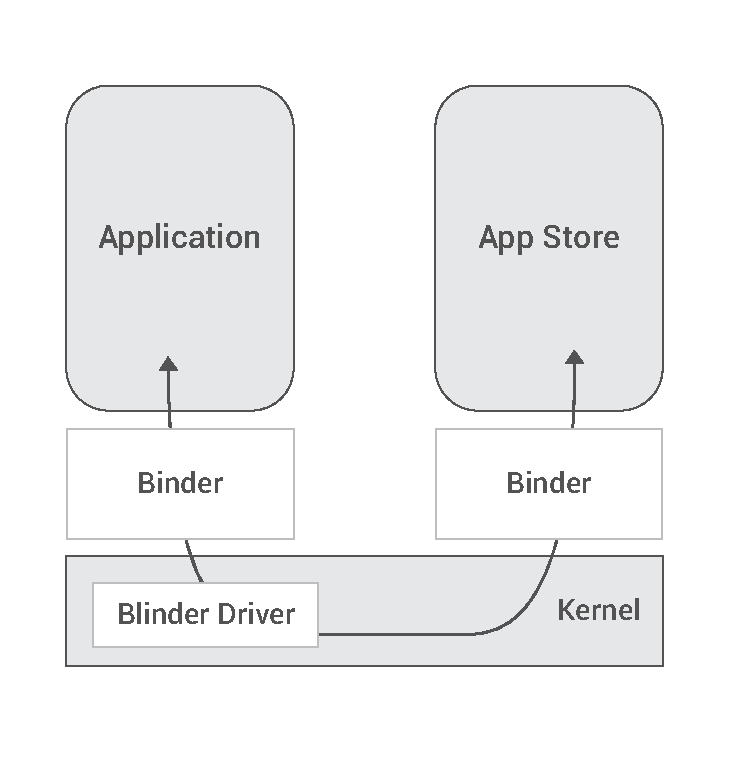
\includegraphics[width=0.5\textwidth]{diagrams/binder_diagram.eps}
\caption{Operating system binder.}
\label{fig:binder}
\end{figure}

Binder framework is a core component in Android architecture and its main goal is to simplify Inter-Process Communication (IPC). Binder is implicitly used whenever an application communicates with OS services or with other applications through Android Java API Framework. The Binder framework will also provide information regarding the Application process which will positively contribute to the App Store Proof-of-Attention reliability.

Once the Application and the App Store's processes are bound, the App Store will periodically verify whether the Application is in the foreground and the User is actively interacting with the device. In order to certify that the User is paying attention to the Application the following conditions should be met:
%are conditions the same as what was previously called requirements?

\begin{itemize}
\item The Application's process must be bound to the App Store's process.
\item The Application must be in foreground.
\item The device screen must be on.
\item The device must not be locked. 
\item The signature of the Application must be verified on the App Store's servers.
\end{itemize}

To assure that the Application's process is bound to App Store, Binder and PackageManager APIs can be used. To verify whether an Application process is in the foreground, both ActivityManager, UserStatsManager and %or?
 PackageManager APIs can be used. To check whether the device screen is on, the PowerManager and Display APIs can be used. Regarding the state of the lock screen, the KeyguardManager API can be used. 

Every application has to be signed by the developer before being installed in an Android's device. App Stores have access to the Applications' signatures and can validate by confirming whether they match with the signature on their servers. If the signature does not match the Application may have been tampered. To obtain the Application's signature, the Binder and PackageManager APIs can be used.

\subsubsection{Limitations client-side}

The proposed solution has some limitations regarding reliability - imposed by Android's inherently insecure environment - and Android API availability - due to Android's version fragmentation and App Store permission level. The use of several different Android APIs can help hardening the solution against an attacker but can not assure full protection against fraud on the client side. In order to mitigate fraud, a system has to have different security layers both on the client side and the server side. 

In Android some APIs are considered sensitive and require system-level permissions to access them. Usually system-level can only be granted to system applications (pre-installed on the device by manufacturers). Also some APIs are only available in certain versions of Android. % The following table summarizes the APIs needed to generate the Proof-of-Attention and their availability:


%\begin{figure}[!ht]
%\centering
%\includegraphics[width=\textwidth]{diagrams/table_android_limitations.eps}
%\caption{Table of Android versions and API support}
%\label{fig:android_versions}
%\end{figure}

The UsageStatsManager requires a System-Level permission but the PACKAGE \_USAGE\_STATS can also be obtained by a normal application if the user explicitly enables it in the Settings.

We can only have an implementation that fulfills all the requirements to certify the the User is paying attention to the Application with a minimum Android version of Jelly Bean (API 16) and above. The Android version limitation is not relevant since that according to Google statistics, only 1.2\% of the Android devices are not running version Jelly Bean (API 16) or above. %reference missing

Also UsageStatsManager is necessary from Lollipop (API 21) onwards requiring that, either the App Store application is a system application, or asking the user to explicitly go to Settings and give the permission. Since in the App Economy the User will be rewarded by the attention given to Applications it will be easy to convince him to manually provide the permission in the case where the App Store is not a system application.


\subsection{Protocol Overview and sketch}


The AppCoins protocol is depicted in figure \ref{fig:design}. It consists in 3 main blocks: Advertising, Deeveloper's Reputation (Rank) and IAB.

\begin{figure}[!ht]
\centering
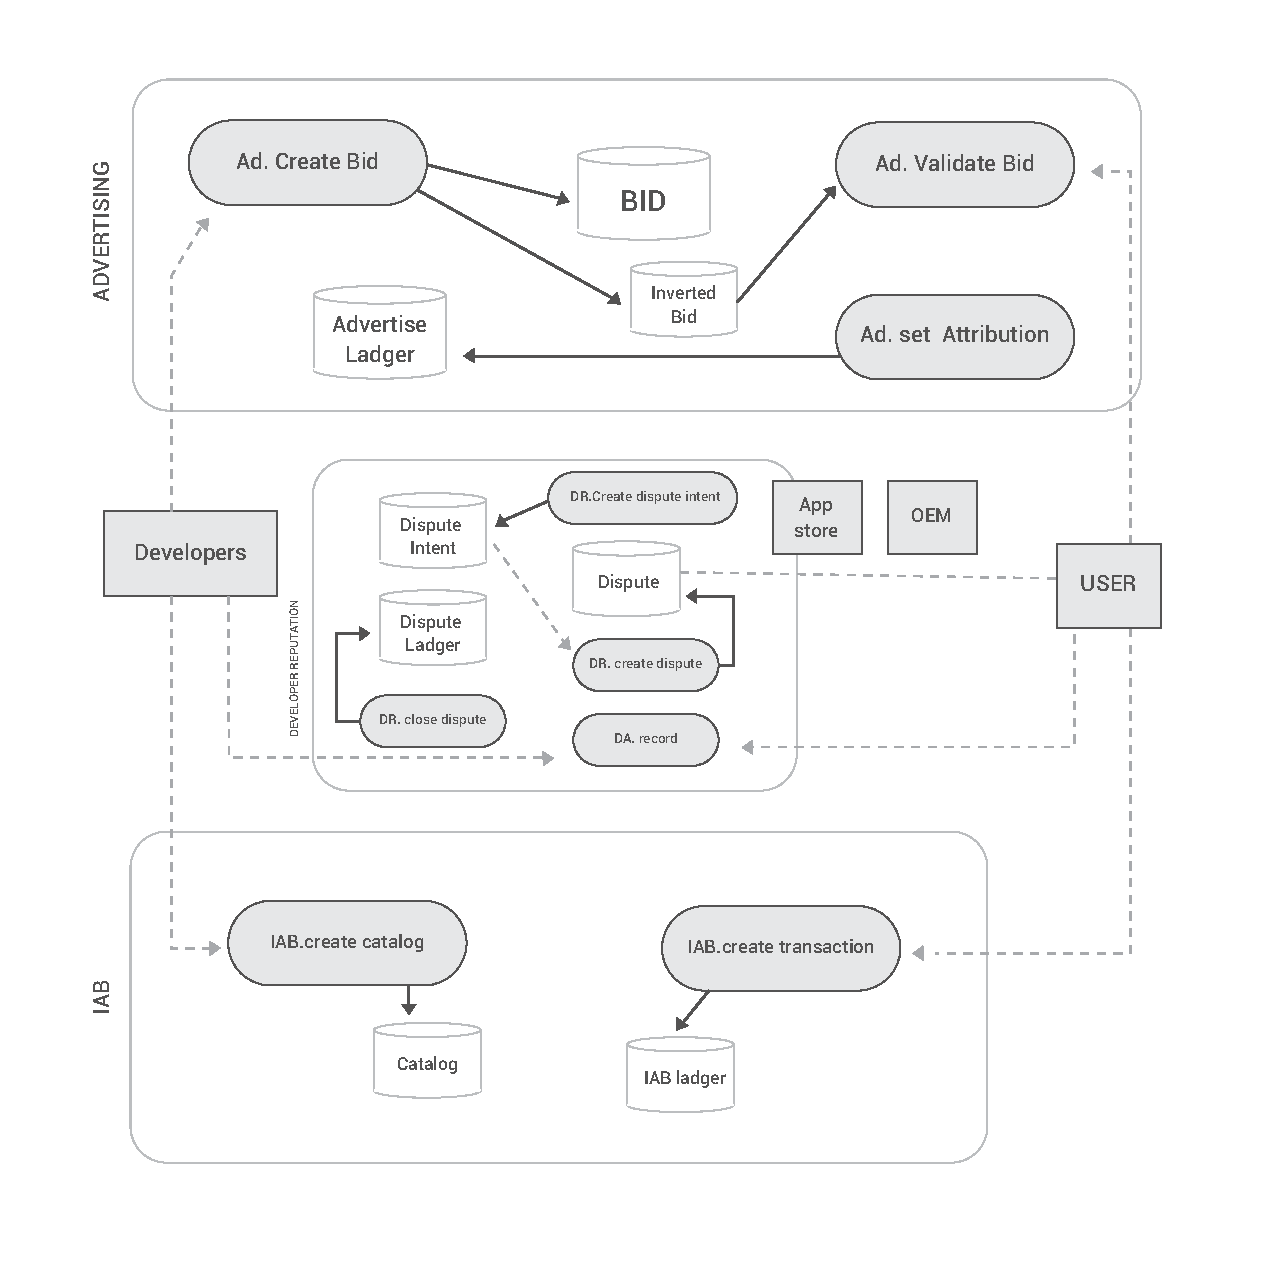
\includegraphics[width=0.7\textwidth]{diagrams/design.eps}
\caption{Overall design of AppCoins and blockchain interactions.}
\label{fig:design}
\end{figure}


Inside each block we see the interactions between the ecosystem players and the blockchain. The rounded squares represent functions / methods of smart contracts and that implement business logic.

The cylinders represents data that is stored in smart contracts own storage or event logs.

\medskip

The Advertising block has 3 functions that interact with three data structures stored in the blockchain: {\em Ad.CreateBid},  {\em Ad.ValidateBid} and  {\em Ad.SetAttribution}. Together, those functions perform the desired behaviour in the Advertising model, ensuring trust and transparency.

The Developer's Reputation block consists functions related with the potential dispute. The blockchain stores three different data structures: the Dispute Intent, the Dispute and the Dispute Leadger.

The IAB has only two functions related with the purchase: IAB.CreateCatalog and IAB.Create Transaction.

In the next section, we will present in detail each of them.


% a diagram that integrates all the players
% the circular but more geek 

%(Include a diagram with the players - component diagram 

% Could be a sequence diagram as in Filecoin diagram 

% (In-App Billing, Advertising, Reputation builder) 

%


